\chapter{Změřené parametry}

\section{Průběh budicího pulzu}
Průběh budicího pulzu byl nejprve změřen osciloskopem Teledyne LeCroy WaveRunner 6 Zi. Tento osciloskop vyniká vzorkovací frekvencí \SI{40}{\gigasample} v reálném čase a analogovou šířkou pásma \SI{4}{\giga\hertz}. Měřicí soustava s tímto osciloskopem je na fotografii \ref{lecroy_photo}. Bohužel v měření na grafu \ref{lecroy} se ukázalo, že šířka pásma \SI{4}{\giga\hertz} je pro toto měření nedostatečná.

\begin{figure}[htbp]
\includegraphics[width=\textwidth,keepaspectratio]{images/measurements/lecroy_photo.jpg}\caption{Fotografie měřicí sestavy s osciloskopem LeCroy Waverunner 6 Zi.}\label{lecroy_photo}
\end{figure}

\begin{figure}[htbp]
\includegraphics[width=\textwidth,keepaspectratio]{images/measurements/lecroy.png}\caption{Náběžná hrana budicího signálu změřená osciloskopem LeCroy Waverunner 6 Zi.}\label{lecroy}
\end{figure}

Následně byl budicí pulz změřen vzorkovací hlavou Agilent 86015C v mainframe Agilent 86100C s měřením v ekvivalentním čase a analogovou šířkou pásma \SI{20}{\giga\hertz}. Pro měření bylo nezbytné připojit jak měřený signál, tak spuštěcí signál. Měřicí soustava je uvedena na fotografii \ref{agilent_photo}. Změřený průběh je uveden v grafu \ref{agilent_fall}. Změřená délka sestupné hrany se pohybuje v rozsahu \SIrange{80}{95}{\pico\second}. Bohužel výrobce u vzorkovací hlavy neuvádí, jaká je nejkratší měřitelná délka náběžné hrany. Proto není možné usuzovat, zda se jedná již o skutečnou délku náběžné hrany, nebo zda je měření zatíženo schopnostmi použité vzorkovací hlavy. Z měření je však možné usuzovat, že délka náběžné hrany je kratší nebo rovna \SI{90}{\pico\second}.
\begin{figure}[htbp]
\includegraphics[width=\textwidth,keepaspectratio]{images/measurements/tdr_photo.jpg}\caption{Fotografie měřicí sestavy s mainframem 86100C.}\label{agilent_photo}
\end{figure}

\begin{figure}[htbp]
\includegraphics[width=\textwidth,keepaspectratio]{images/measurements/agilent_fall.png}\caption{Měření sestupné hrany na mainframe Agilent 86100C.}\label{agilent_fall}
\end{figure}

\section{Parametry fázového závěsu}
Snahou v této části měření bylo změřit fázový šum fázového závěsu. Tato snaha bohužel byla z větší části neúspěšná. Nejprve byl vyzkoušen osciloskop Teledyne LeCroy WaveRunner 6 Zi, který umí měřit fázový šum a ze změřených dat vytvořit graf histogramu fázového šumu, graf frekenčního spektra šumu a numerické statistiky. Bohužel se ukázalo, že tento osciloskop, který katedra elektromagnetickéh pole vlastní, není vybaven softwarovou licencí na tato měření. Vyzkoušen byl tedy mainframe Agilent DCA-J 86100C, který podle označení DCA-J obsahuje hardwarové vybavení potřebné pro měření jitteru. Bohužel i u tohoto osciloskopu se také ukázalo, že není vybaven softwarovou licencí pro tato měření. Bez této licence je schopen pouze zobrazit dvě statistické hodnoty, mezivrcholovou úroveň fázového šumu a efektivní úroveň fázového šumu. Nakonec byl pouze změřen fázový šum mezi dvěma výstupy připojenými ke stejnému fázovému závěsu. Výsledkem měření je tedy fázový šum odpovídající šumu mezi dvěma výstupy diferenciálního páru. Toto měření je vidět na grafu \ref{agilent_fall}. Mezikanálový šum tedy dosahuje mezivrcholové úrovně \SI{21}{\pico\second} a efektivní úrovně \SI{3.4}{\pico\second}.

\section{TDR měření vstupní impedance reflektometru}
Vstupní impedance reflektometru byla změřena pomocí TDR hlavy Agilent 54754A v mainframe Agilent 86100C. Před použitím byla provedena kompletní kalibrace TDR hlavy pomocí kalibrů open, short a match. Podle očekávání na přechodu mezi konektorem a plošným spojem dochází k poklesu impedance přibližně na \SI{35}{\ohm}. K dalšímu poklesu impedance dochází nejspíše na přechodu mezi koplanárním vedení pod konektorem a úzkým koplanárním vedením. Dále již impedance reflektometru odpovídá \SI{50}{\ohm}.
\begin{figure}[htbp]
\includegraphics[width=\textwidth,keepaspectratio]{images/measurements/tdr_profile.png}\caption{TDR měření vstupní impedance reflektometru.}\label{tdr_profile}
\end{figure}

\section{Měření vstupní impedance reflektometru pomocí VNA}
Měření impedance bylo zopakováno pomocí \acrshort{VNA} Agilent E8364A. Výsledek měření je prezentován v grafu \ref{vna_impedance}. Parametr $S_{11}$ je menší než \SI{-20}{\deci\bel} pro frekvence do \SI{3.5}{\giga\hertz} a menší než \SI{-10}{\deci\bel} pro frekvence do \SI{7.7}{\giga\hertz}. Měření bylo provedeno při různých výkonech generátoru ve VNA za účelem zjištění, zda se vstupní port chová lineárně. Test probíhal pro výkony do \SI{0}{\deci\bel m}, neprojevovaly se žádné viditelné nelineární jevy.

Toto měření bylo opakováno s neosazenou deskou plošných spojů z obr. \ref{pcb_coplanar}, změřený průběh parametru $S_{11}$ je v grafu \ref{vna_impedance_blank}. Změřený průběh je velmi podobný osazené desce plošných spojů, charakteristické prvky se vyskytují na podobných frekvencích a s podobnou velikostí. Zavěrem tohoto měření je tedy fakt, že špatné přizpůsobení vstupu není způsobeno navrženým splitterem, budičem, ani vzorkovačem, nýbrž nesprávným návrhem vedení pod konektorem a nekvalitním konektorem.

\begin{figure}[htbp]
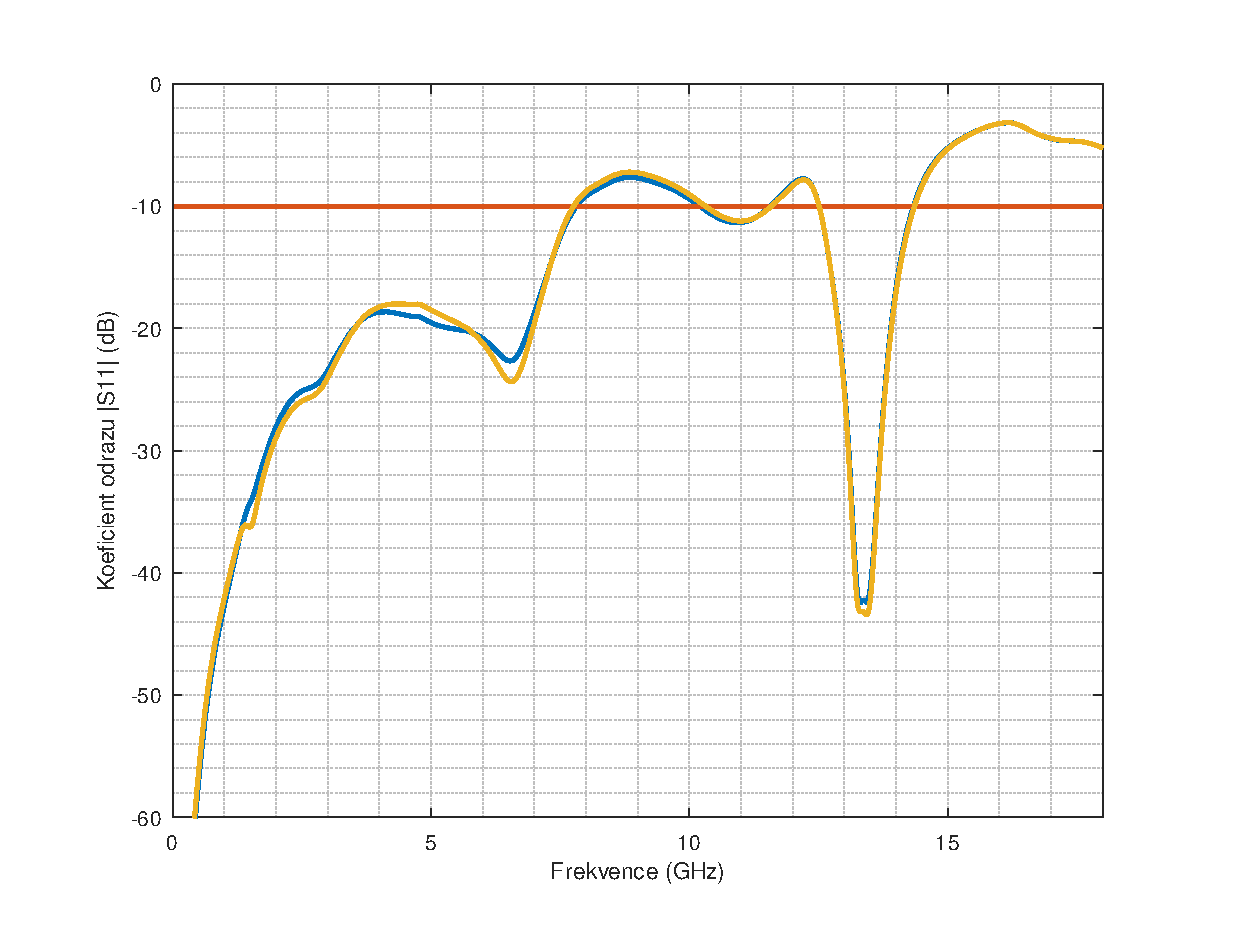
\includegraphics[width=\textwidth,keepaspectratio]{images/measurements/vna_high_low.eps}\caption{Měření vstupní impedance reflektometru pomocí VNA. Modře je označeno měření v logické úrovni 1 a žlutě měření v logické úrovni 0.}\label{vna_impedance}
\end{figure}

\begin{figure}[htbp]
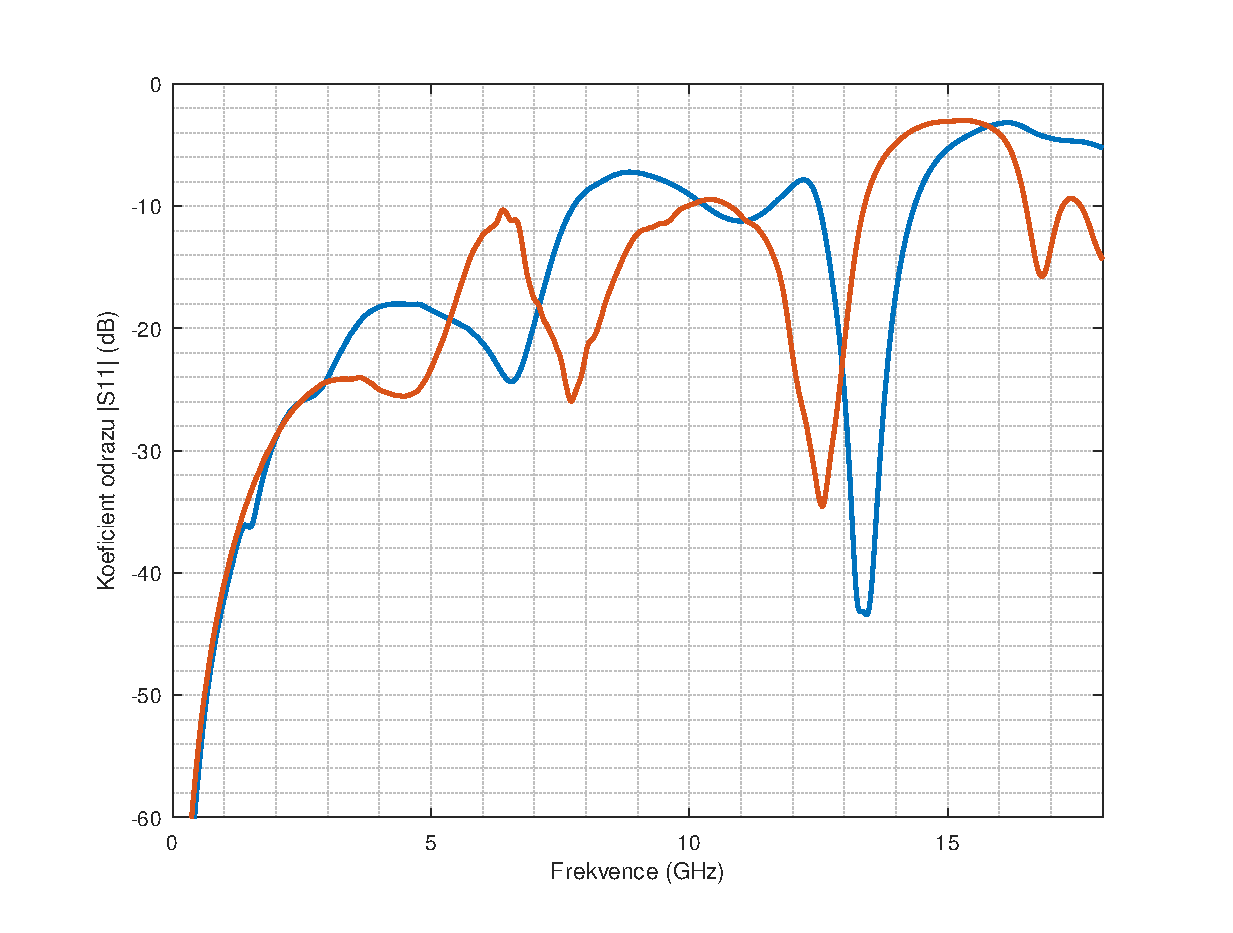
\includegraphics[width=\textwidth,keepaspectratio]{images/measurements/vna_low_blank.eps}\caption{Měření vstupní impedance reflektometru pomocí VNA. Modře je označeno měření v logické úrovni 0, červeně měření na neosazené desce z obr. \ref{pcb_coplanar} terminované \SI{50}{\ohm} terminátorem.}\label{vna_impedance_blank}
\end{figure}

\section{Měření parametrů použitého substrátu}
Pro ověření permitivity použitého substrátu byla vytvořena testovací deska s kalibry pro kalibrační metody \acrshort{TRL} a \acrshort{UOSM}. Tato deska je na fotografii \ref{uoml}. Nachází se na ní seshora postupně kalibrační vedení nulové délky \quotedblbase thru\textquotedblleft , kalibry \quotedblbase short\textquotedblleft , \quotedblbase open\textquotedblleft{} a \quotedblbase match\textquotedblleft{}. Pod nimi se nachází tři vedení různých délek. Seshora jsou to vedení délek \SI{8}{\milli\meter}, \SI{50}{\milli\meter} a \SI{69.8}{\milli\meter}. Tloušťka substrátu a povrchová úprava je stejná jako u reflektometru, tedy \SI{0.6}{\milli\meter} a olovnatý HAL. Deska byla navržena tak, aby bylo možné na ni namontovat jak kvalitní konektory Southwest Endlaunch, tak i připájet levné konektory použité na reflektometru. Detail kalibru \quotedblbase match\textquotedblleft{} v podobě rezistoru velikosti 0201 je na fotografii \ref{match_detail}, pro srovnání velikosti má otvor napravo od rezistoru průměr \SI{0.3}{\milli\meter}.
\begin{figure}[htbp]
\includegraphics[width=\textwidth,keepaspectratio]{images/measurements/match.jpg}\caption{Detail kalibru \quotedblbase match\textquotedblleft .}\label{match_detail}
\end{figure}

\begin{figure}[htbp]
\includegraphics[width=\textwidth,keepaspectratio]{images/measurements/uoml.jpg}\caption{Testovací deska plošných spojů pro změření parametrů substrátu s připájenými konektory.}\label{uoml}
\end{figure}

Pro zjištění parametrů substrátu bylo provedeno měření všech vedení a kalibrů pomocí \acrshort{VNA} Agilent E8364A. Změřená data byla zpracována pomocí algoritmu, který vytvořil podle \cite{TRL_calibration} Ing.~Viktor Adler,~Ph.D. v matematickém prostředí MATLAB. Takto zpracovaná data ze změřených kalibrů, vedení a jejich vzájemných kombinací byla použita pro kalibraci. Pomocí takto získané kalibrace byly získány parametry jednoho z vedení. Tato data byla následně importována do simulačního nástroje CST a pomocí optimalizace parametrů substrátu byly získány jeho vlastnosti. Bohužel takto získané parametry jsou zatíženy zdrojem chyb, který pramení ze skutečnosti, že byly získávány pouze parametry substrátu, nebyl uvažován vliv samotného vedení. Ztráty způsobené např. hrubostí povrchu vedení na desce plošných spojů jsou tak součástí získaných parametrů substrátu. Parametr $\tan \delta$ uvedený v tabulce \ref{permittivity_table} tedy nejspíše neodpovídá přesně ztrátám způsobeným substrátem. V tabulce \ref{permittivity_table} je vidět, že permitivita substrátu je až do \SI{6}{\giga\hertz} přibližně konstantní, poté začne klesat. Pokles je ovšem vcelku malý, na \SI{18}{\giga\hertz} činí pokles permitivity méně než \SI{1.5}{\percent}.

Při permitivitě substrátu $\epsilon'=\SI{4.1}{}$ místo $\epsilon'=\SI{4.6}{}$, se kterou byl reflektometr navržen, tak vychází impedance použitého koplanárního vedení na přibližně \SI{52.5}{\ohm}. Vzhledem ke skutečnosti, že pod testovacím konektorem se nachází vedení s nesprávnou (nižší) impedancí, má tento fakt vliv spíše pozitivní, protože je tak výsledný odraz na měřicím portu menší, než bylo původně očekáváno.

\begin{table}[htbp]
\begin{center}
\caption{Tabulka permitivity a ztrát substrátu získaná z testovací desky plošných spojů z obr. \ref{uoml}}\label{permittivity_table}
\begin{tabular}{ |c|c|c|  }
 \hline
 Frekvence (\si{\giga\hertz}) & $\epsilon'$ (-) & $\tan \delta$ (-)\\
 \hline
 \hline
	\SI{0.99}{}	&	\SI{4.100}{}	&	\SI{0.013}{}\\
 \hline
	\SI{2.18}{}	&	\SI{4.104}{}	&	\SI{0.006}{}\\
 \hline
	\SI{4.15}{}	&	\SI{4.081}{}	&	\SI{0.005}{}\\
 \hline
	\SI{6.13}{}	&	\SI{4.096}{}	&	\SI{0.007}{}\\
 \hline
	\SI{8.10}{}	&	\SI{4.065}{}	&	\SI{0.010}{}\\
 \hline
	\SI{10.1}{}	&	\SI{4.083}{}	&	\SI{0.012}{}\\
 \hline
	\SI{12.1}{}	&	\SI{4.050}{}	&	\SI{0.014}{}\\
 \hline
	\SI{14.0}{}	&	\SI{4.061}{}	&	\SI{0.015}{}\\
 \hline
	\SI{16.0}{}	&	\SI{4.037}{}	&	\SI{0.017}{}\\
 \hline
	\SI{18.0}{}	&	\SI{4.046}{}	&	\SI{0.017}{}\\
 \hline
\end{tabular}
\end{center}
\end{table}

\section{Parametry změřených dat}
Prvním zajímavým parametrem, který je možné z dat změřených reflektometrem získat, je délka měřené náběžné hrany. V grafu \ref{measured_open_risetime} je tato náběžná hrana vykreslena. Při měření délky náběžné hrany mezi \SIrange{20}{80}{\percent} mezi počátečním a konečným napětím je tato délka \SI{220}{\pico\second}. Celý změřený průběh pro kalibr \quotedblbase open\textquotedblleft{} na konci vedení je zakreslen v grafu \ref{measured_open}. Z grafu je vidět, že koeficient odrazu na tomto kalibru je $\Gamma \doteq 1$. Ve vzdálenosti odpovídající délce kabelu mezi reflektometrem a kalibrem, tedy přibližně okolo \SI{23}{\nano\second} se nachází další odraz, tentokrát menší a záporný. Ten je způsoben odrazem změřené odezvy na kalibr od konektoru reflektometru a zpět. Záporný je z toho důvodu, že impedance měřicího portu reflektometru je menší než \SI{50}{\ohm}.
\begin{figure}[htbp]
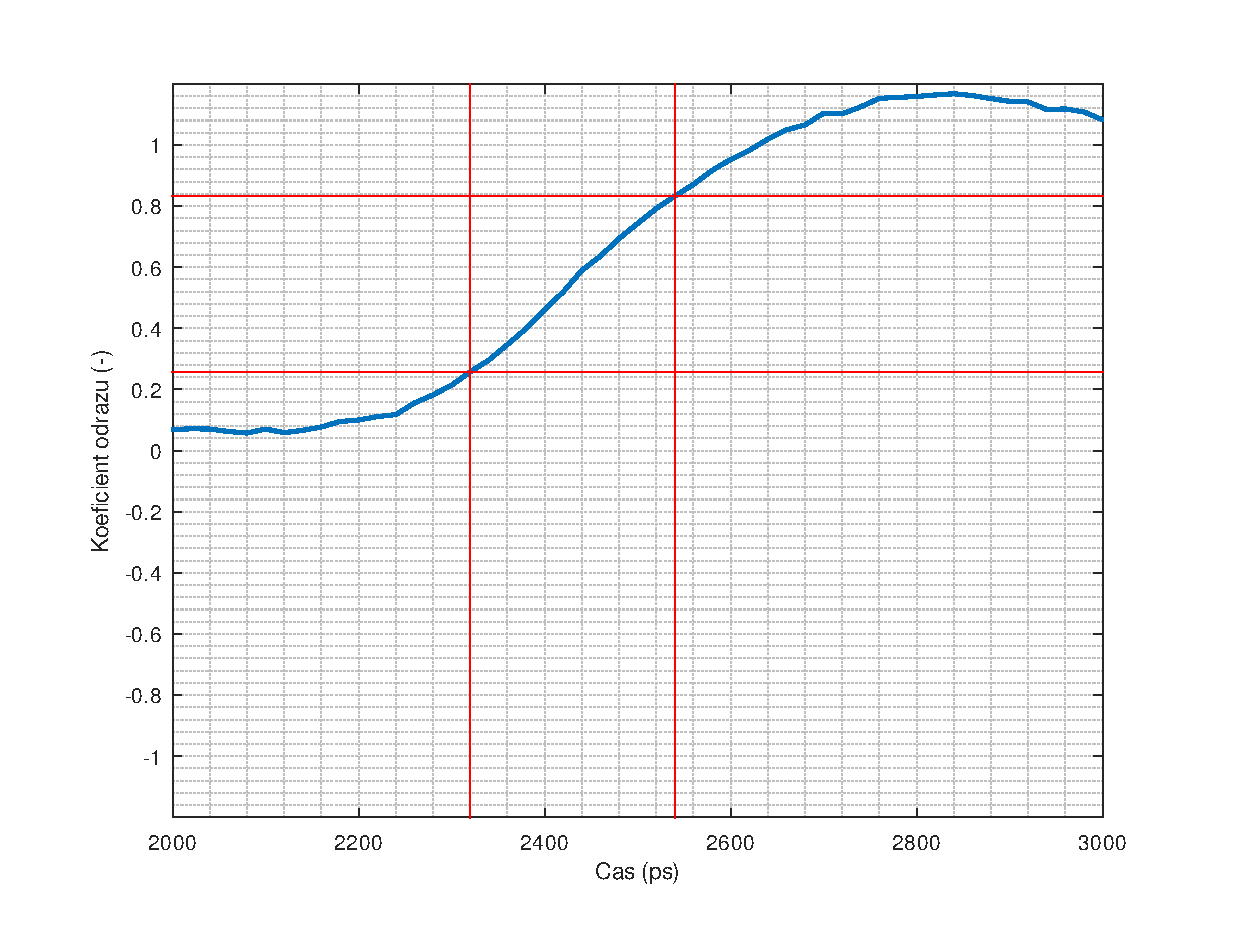
\includegraphics[width=\textwidth,keepaspectratio]{images/self-measurements/measure_open_risetime.eps}\caption{Délka náběžné hrany při měření kalibru \quotedblbase open\textquotedblleft{} na konci vedení.}\label{measured_open_risetime}
\end{figure}

\begin{figure}[htbp]
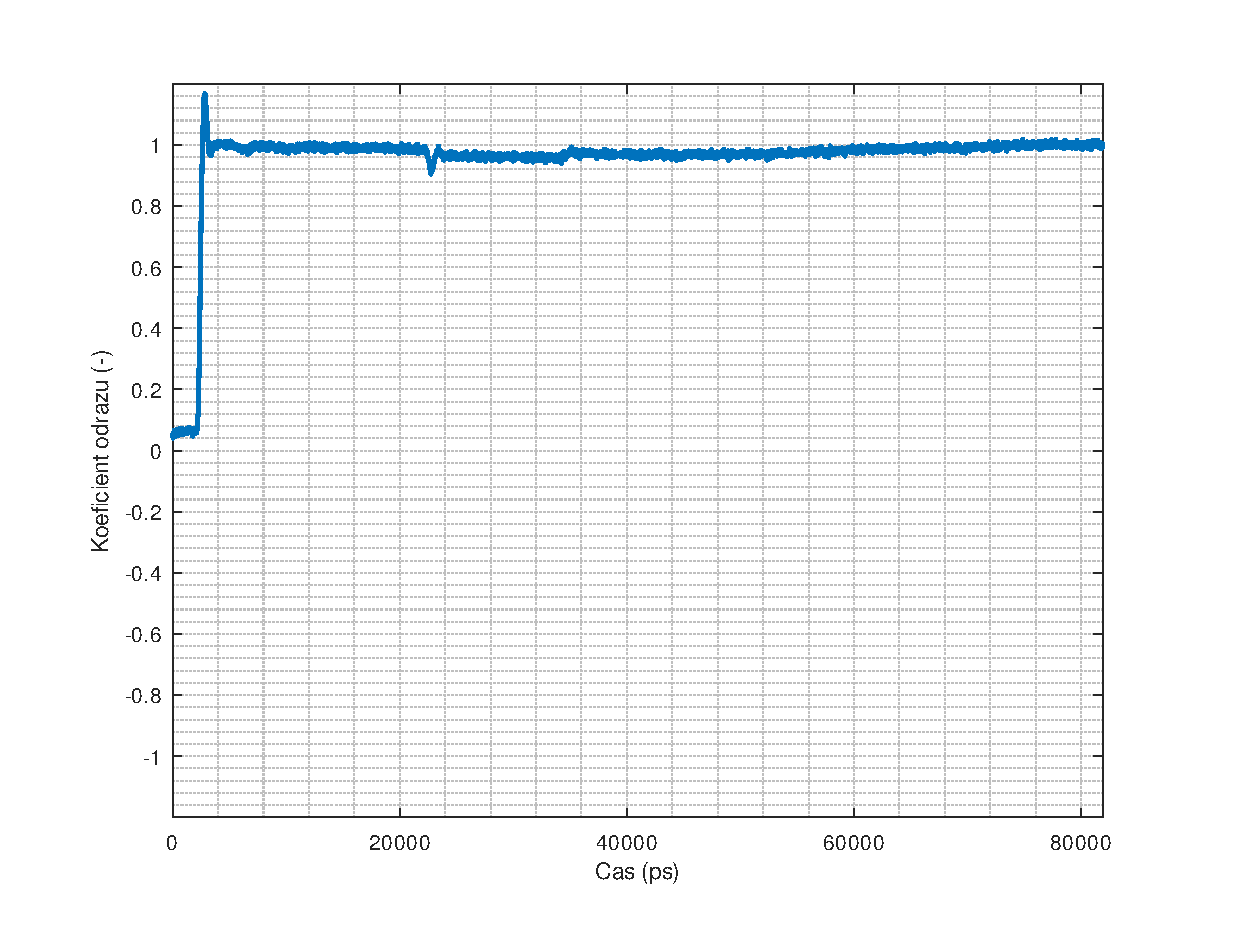
\includegraphics[width=\textwidth,keepaspectratio]{images/self-measurements/measured_open.eps}\caption{Odezva při měření kalibru \quotedblbase open\textquotedblleft{} na konci vedení.}\label{measured_open}
\end{figure}

Při měření kalibru v grafu \ref{measured_short_risetime} \quotedblbase short\textquotedblleft{} je náběžná hrana odezvy dlouhá \SI{240}{\pico\second}. Celá odezva se po diskontinuitě pohybuje okolo koeficientu odrazu $\Gamma \doteq -1$. Opět je na grafu \ref{measured_short} tento nežádoucí odraz vidět přibližně na \SI{23}{\nano\second}. Tentokrát má ovšem stejnou polaritu jako odraz od kalibru, protože koeficient odrazu měřicího portu i kalibru je záporný, po dvou odrazech má tedy stejnou polaritu jako první odraz.

\begin{figure}[htbp]
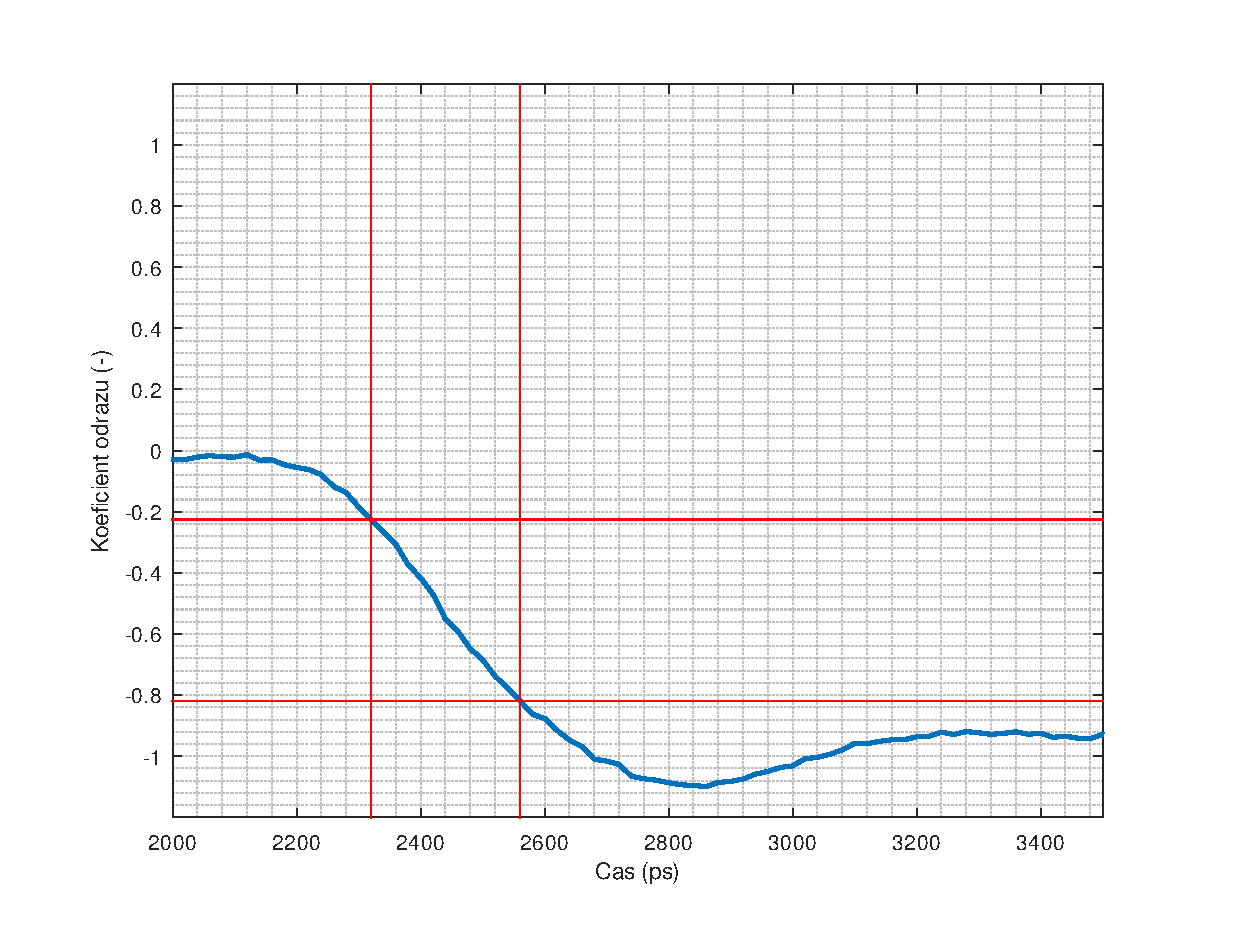
\includegraphics[width=\textwidth,keepaspectratio]{images/self-measurements/measure_short_risetime.eps}\caption{Délka náběžné hrany při měření kalibru \quotedblbase short\textquotedblleft{} na konci vedení.}\label{measured_short_risetime}
\end{figure}

\begin{figure}[htbp]
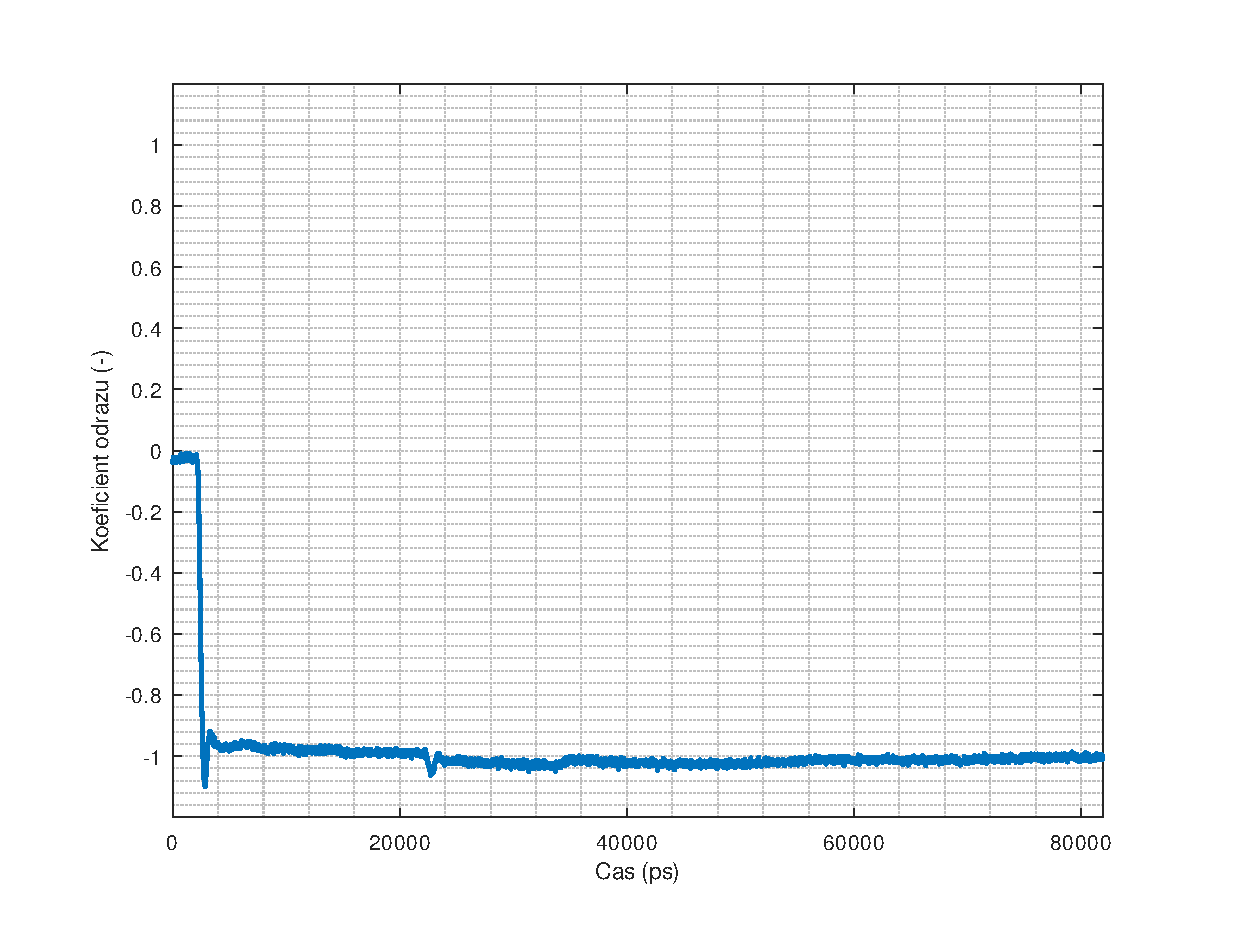
\includegraphics[width=\textwidth,keepaspectratio]{images/self-measurements/measured_short.eps}\caption{Odezva při měření kalibru \quotedblbase short\textquotedblleft{} na konci vedení.}\label{measured_short}
\end{figure}

Odezva na kalibr \quotedblbase match\textquotedblleft{} je v grafu \ref{measured_load}. Dle očekávání není v změřených datech viditelný žádný odraz od tohoto kalibru, přítomen je pouze šum.

\begin{figure}[htbp]
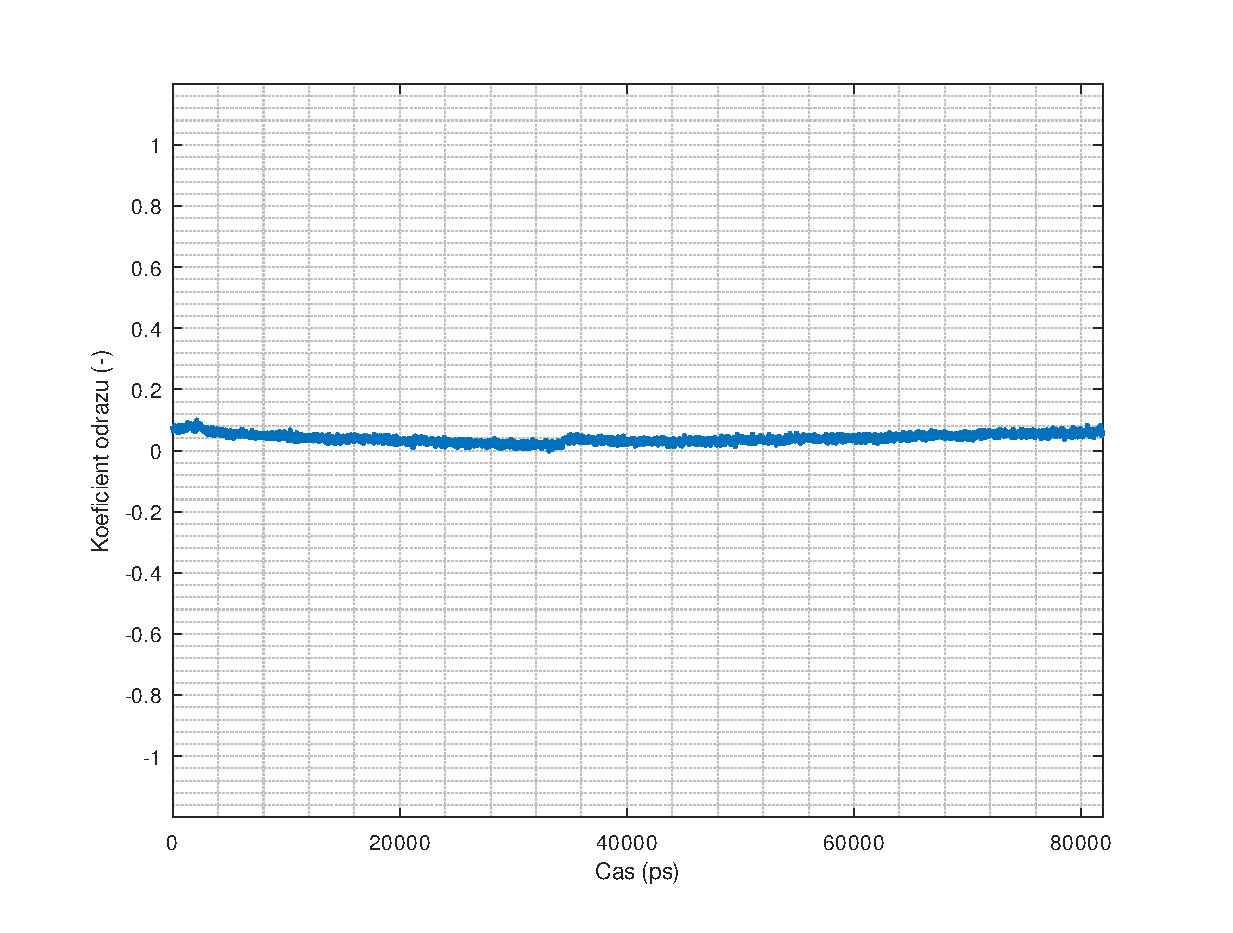
\includegraphics[width=\textwidth,keepaspectratio]{images/self-measurements/measured_load.eps}\caption{Odezva při měření kalibru \quotedblbase match\textquotedblleft{} na konci vedení.}\label{measured_load}
\end{figure}

\section{Měření funkčnosti potlačení šumu a zvlnění průměrováním a jednoduchou kalibrací}
Pro ověření funkčnosti potlačení šumu pomocí průměrování byl změřen kalibr \quotedblbase open\textquotedblleft{} při různých počtech průměrování ($1\times$, $2\times$, $4\times$, $8\times$, $16\times$, $32\times$, $64\times$). Tato změřená data jsou zanesena v grafu \ref{noise_raw_comparison}. Graf je pouze informativní, data pro různé úrovně průměrování jsou posunuta tak, aby se nepřekrývala. Měření probíhalo při vzorkovacím kroku $10\times$~větším, než ve zbytku práce, tedy přibližně \SI{196.2}{\pico\second}. Byl změřen i standard \quotedblbase load\textquotedblleft{} při průměrování $64\times$, pomocí získaných dat byla zkalibrována data jednotlivých měření kalibru \quotedblbase open\textquotedblleft . Z měření je vidět, že úroveň šumu klesá s rostoucím počtem průměrování, přičemž nedochází k žádným viditelným negativním jevům průměrování, jako je například prodloužení náběžné hrany vlivem vysokého fázového šumu. V grafu \ref{noise_cal_comparison} jsou zakreslena tatáž změřená data po kalibraci pomocí standardu \quotedblbase load\textquotedblleft . Z tohoto grafu je vidět, že téměř veškeré zvlnění měřeného signálu pomocí této kalibrace bylo výrazně potlačeno.

\begin{figure}[htbp]
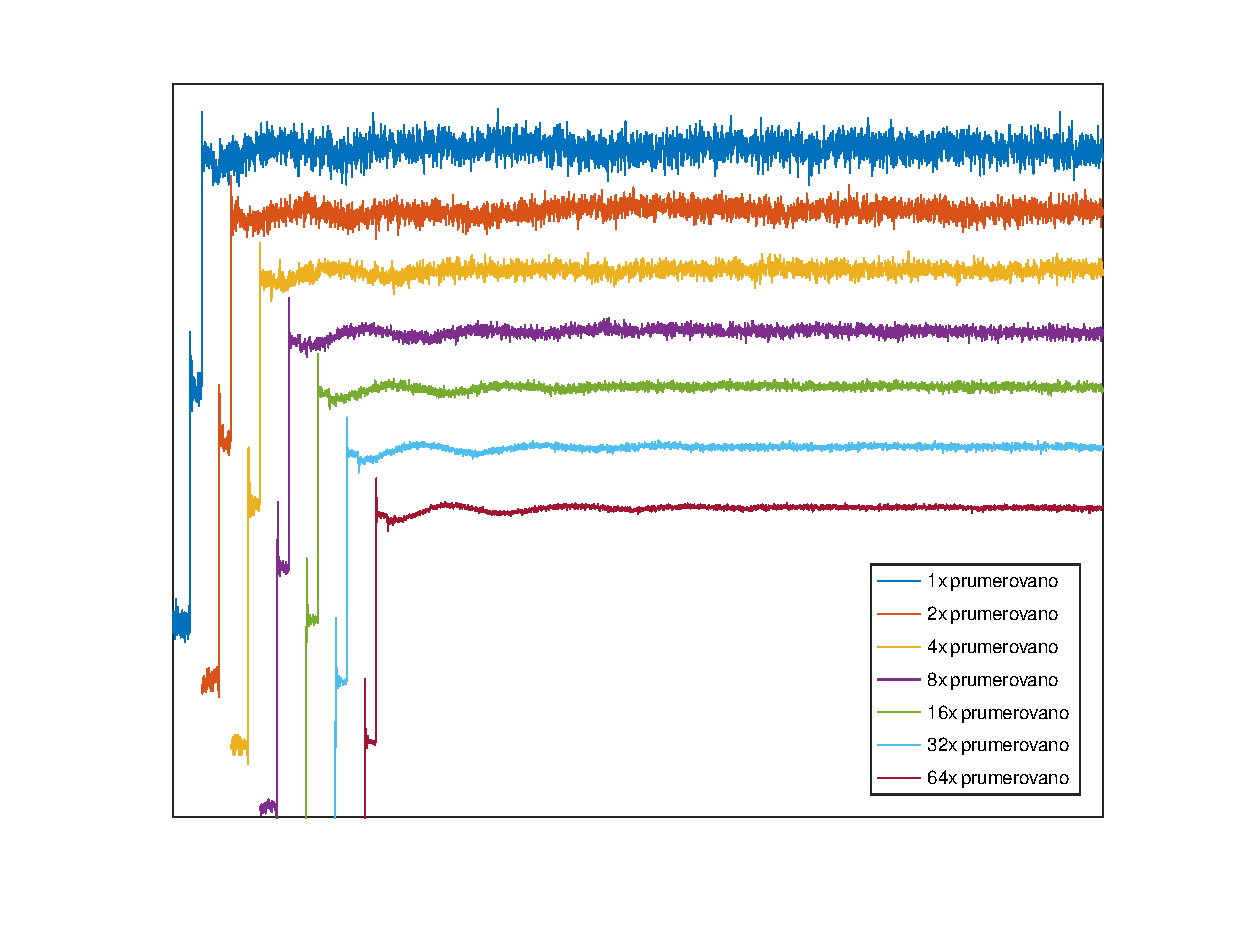
\includegraphics[width=\textwidth,keepaspectratio]{images/noise_raw_comparison.eps}\caption{Porovnání úrovně šumu pro různé počty průměrování, bez jednoduché kalibrace pomocí standardu \quotedblbase load\textquotedblleft .}\label{noise_raw_comparison}
\end{figure}

\begin{figure}[htbp]
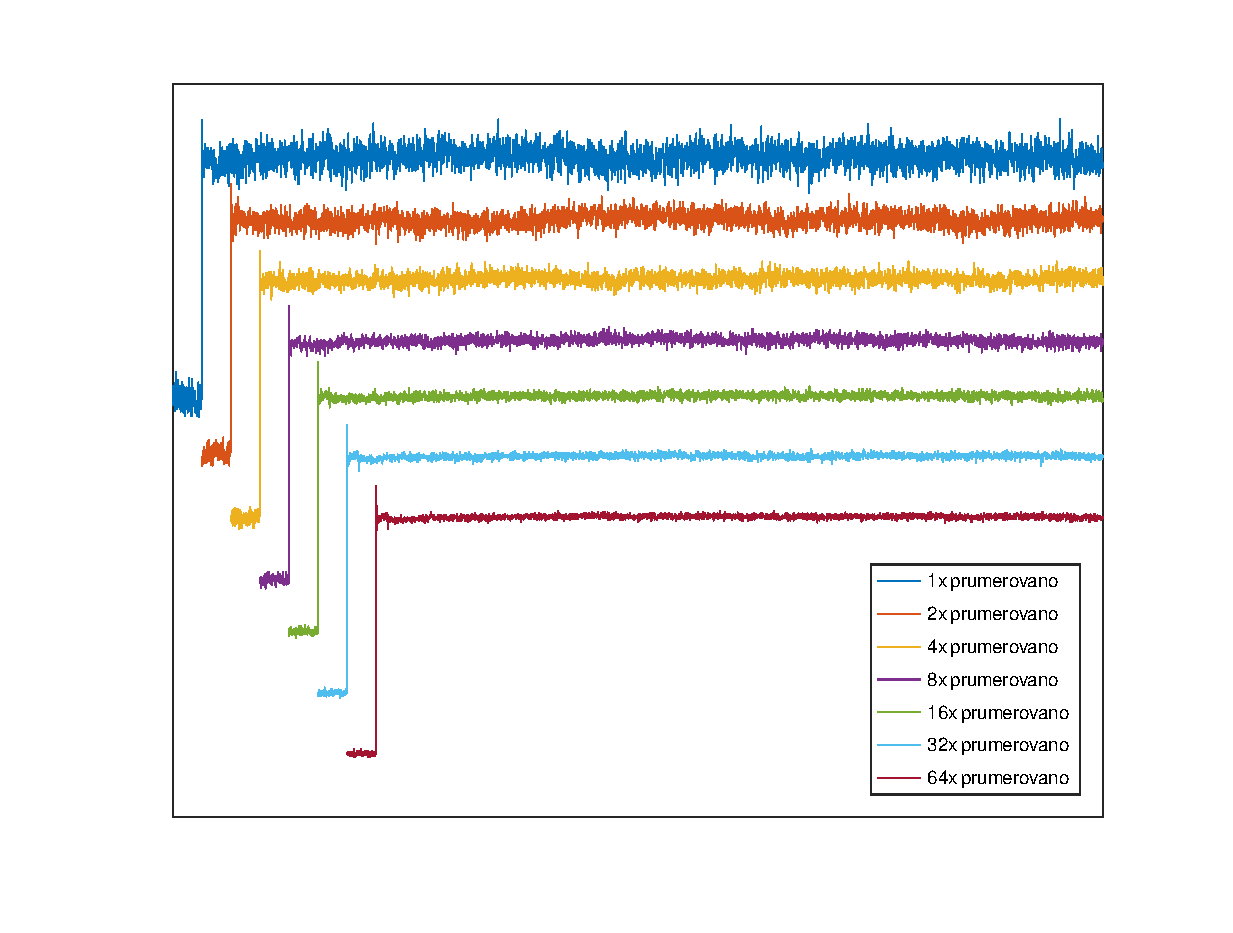
\includegraphics[width=\textwidth,keepaspectratio]{images/noise_cal_comparison.eps}\caption{Porovnání úrovně šumu pro různé počty průměrování, s použitím jednoduché kalibrace pomocí standardu \quotedblbase load\textquotedblleft .}\label{noise_cal_comparison}
\end{figure}

\begin{figure}[htbp]
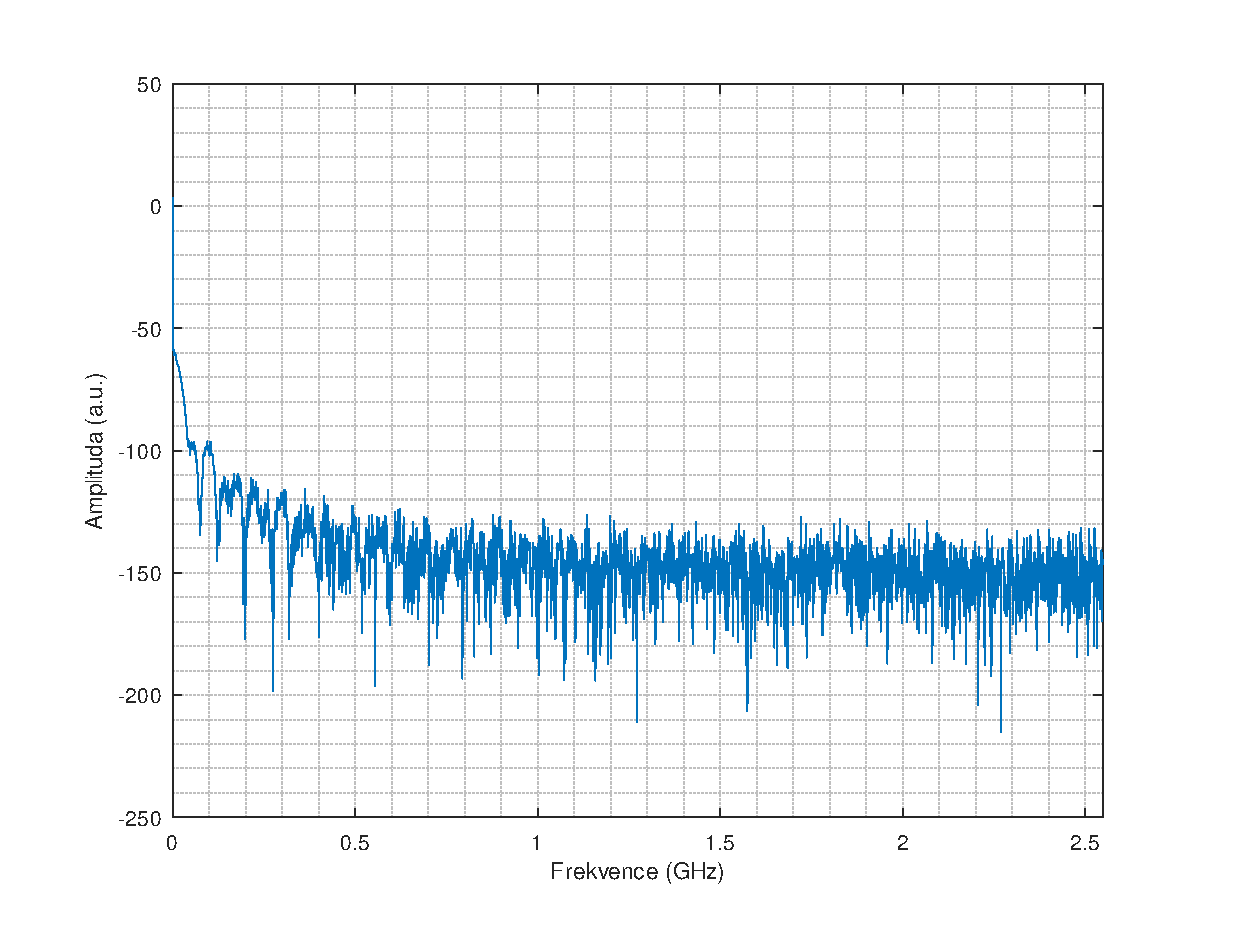
\includegraphics[width=\textwidth,keepaspectratio]{images/noise_raw_avg1.eps}\caption{Spektrum měřeného kalibru \quotedblbase open\textquotedblleft{} při průměrování $1\times$, bez jednoduché kalibrace pomocí standardu \quotedblbase load\textquotedblleft .}\label{noise_raw_avg1}
\end{figure}

\begin{figure}[htbp]
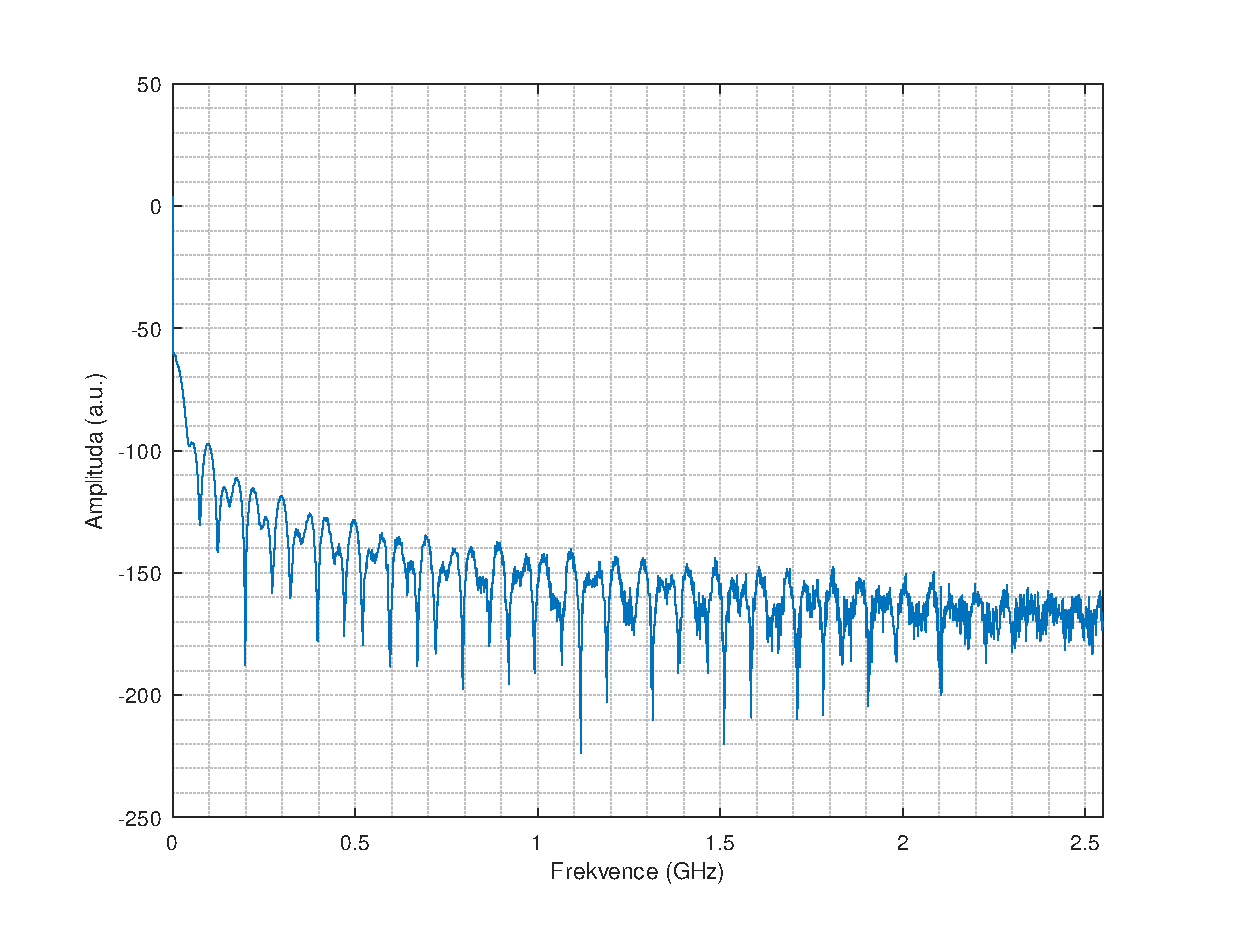
\includegraphics[width=\textwidth,keepaspectratio]{images/noise_raw_avg64.eps}\caption{Spektrum měřeného kalibru \quotedblbase open\textquotedblleft{} při průměrování $64\times$, bez jednoduché kalibrace pomocí standardu \quotedblbase load\textquotedblleft .}\label{noise_raw_avg64}
\end{figure}

\begin{figure}[htbp]
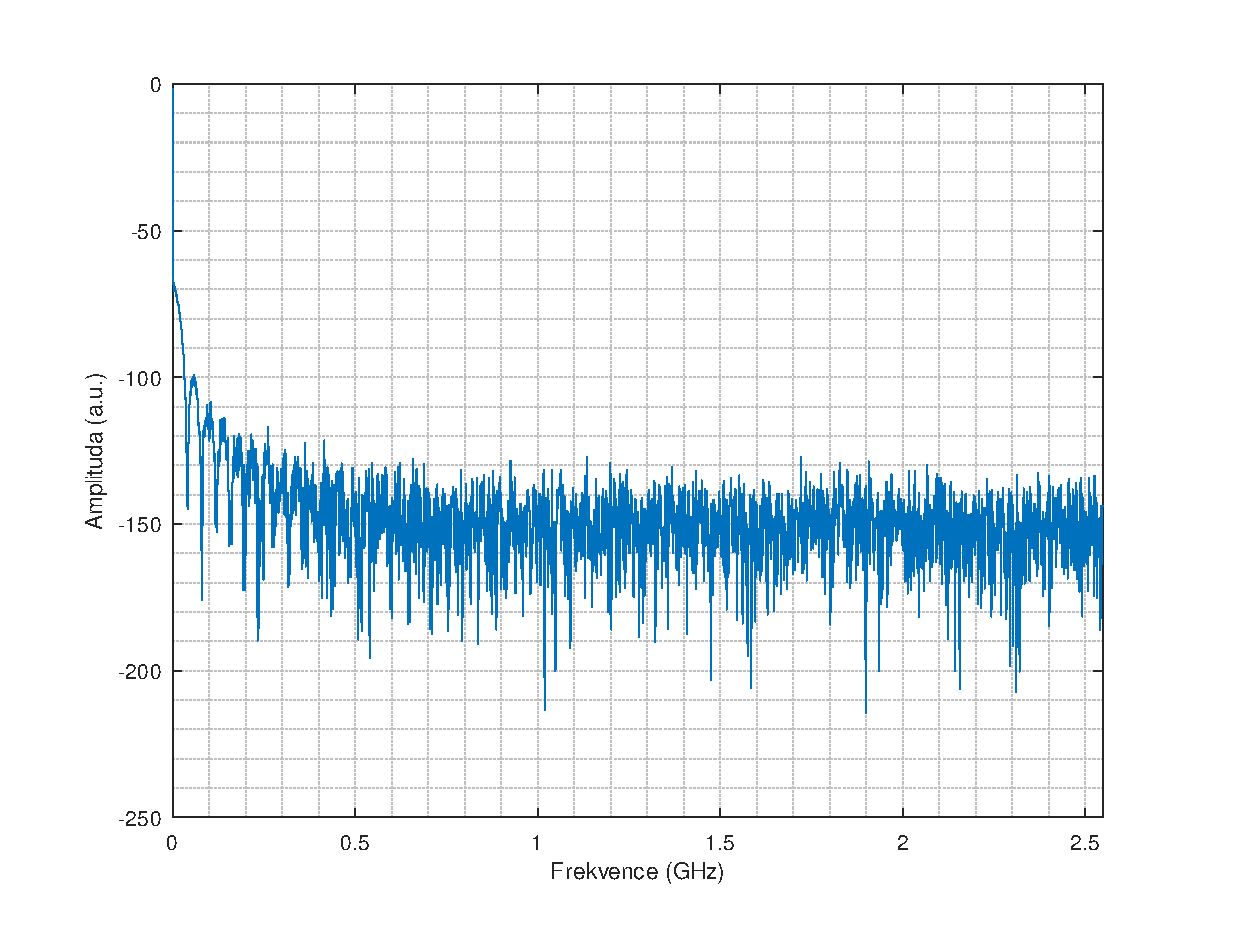
\includegraphics[width=\textwidth,keepaspectratio]{images/noise_cal_avg1.eps}\caption{Spektrum měřeného kalibru \quotedblbase open\textquotedblleft{} při průměrování $1\times$, s použitím jednoduché kalibrace pomocí standardu \quotedblbase load\textquotedblleft .}\label{noise_cal_avg1}
\end{figure}

\begin{figure}[htbp]
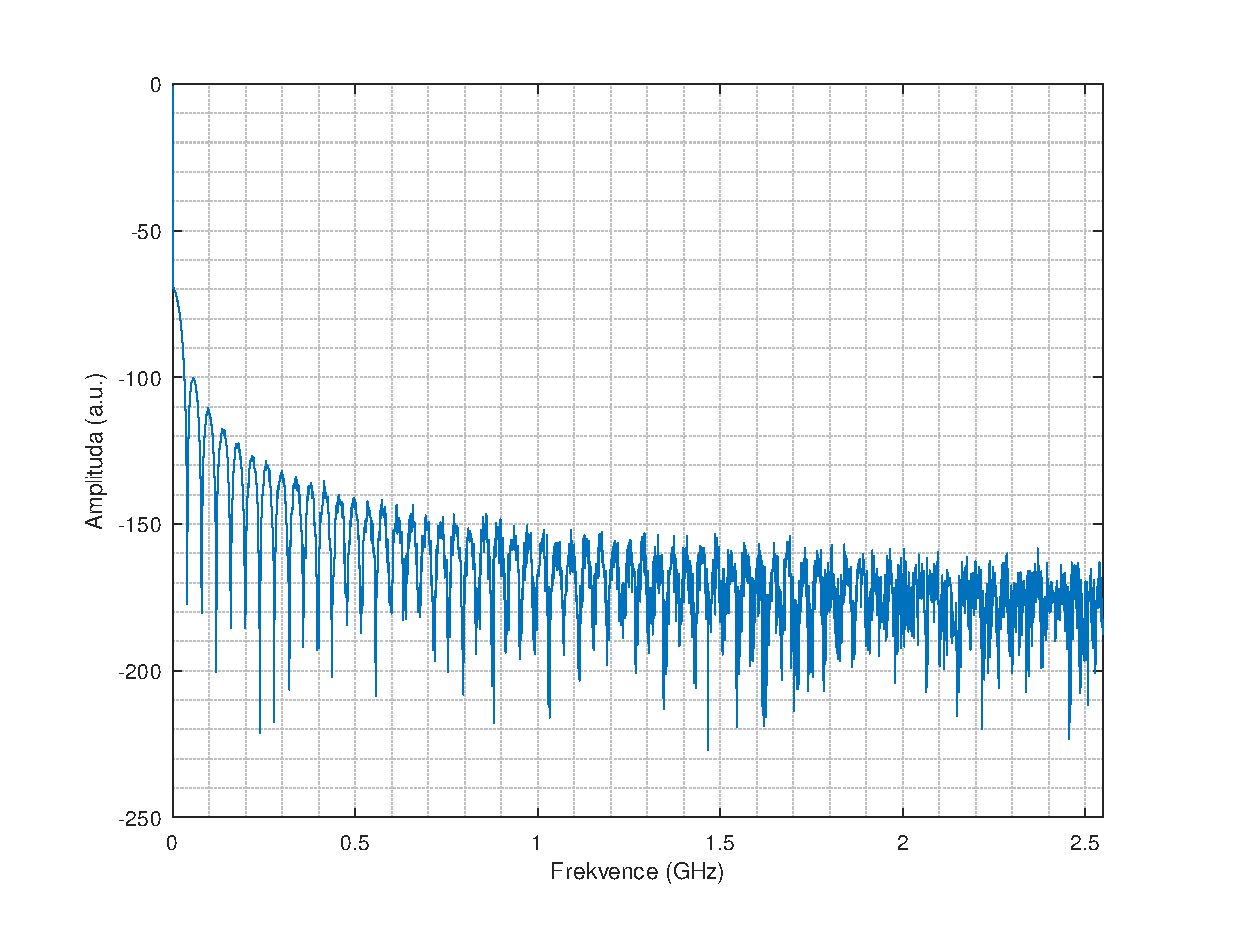
\includegraphics[width=\textwidth,keepaspectratio]{images/noise_cal_avg64.eps}\caption{Spektrum měřeného kalibru \quotedblbase open\textquotedblleft{} při průměrování $64\times$, s použitím jednoduché kalibrace pomocí standardu \quotedblbase load\textquotedblleft .}\label{noise_cal_avg64}
\end{figure}


Amplitudové spektrum měřeného kalibru při počtech průměrování $1\times$ a $64\times$, s jednoduchou kalibrací i bez ní, je uvedeno v grafech \ref{noise_raw_avg1}, \ref{noise_raw_avg64}, \ref{noise_cal_avg1} a \ref{noise_cal_avg64}. V grafu \ref{noise_raw_avg64} je oproti grafu \ref{noise_raw_avg1} vidět výrazně nižší úroveň šumu - spektrum je hladší a i na frekvencích přes \SI{2}{\giga\hertz} jsou vidět periodické propady ve spektru, zatímco bez průměrování jsou tyto propady viditelné jen přibližně do \SI{0.5}{\giga\hertz}. Pomocí průměrování tedy bylo dosaženo snížení šumové úrovně a rozšíření použitelného frekvenčního rozsahu reflektometru. Graf \ref{noise_cal_avg1} a \ref{noise_raw_avg1} vypadají podobně, pro malé počty průměrování tedy kalibrace nepřínáší výrazné vylepšení měřených dat. V grafu \ref{noise_cal_avg64} je však vidět, že při velkém počtu průměrování zlepšuje kalibrace dynamický rozsah. Při použití kalibrace je amplituda mezi vrcholy a propady ve spektru přibližně \SIrange{80}{90}{\deci\bel}, bez použití kalibrace je tato amplituda pouze přibližně \SIrange{40}{80}{\deci\bel}.

Experimentálně tedy bylo zjištěno, že průměrováním a kalibrací pomocí kalibru \quotedblbase load\textquotedblleft{} je možné výrazně potlačit šum a zvlnění a zlepšit dynamický rozsah měření.
